\begin{figure}
  \center{
  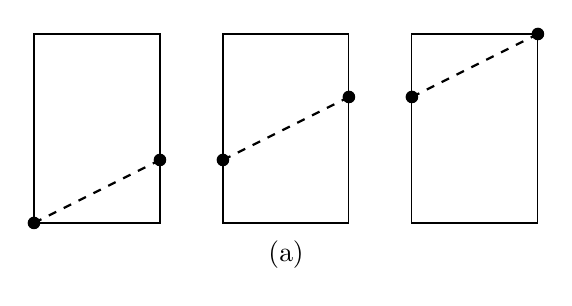
\begin{tikzpicture}[scale=0.8]
    \draw (0,0) rectangle ++(2,3);
    \draw[dashed,thick] (0,0) -- ++(2,1);
    \fill (0,0) circle (0.1);
    \fill (2,1) circle (0.1);

    \draw (3,0) rectangle ++(2,3);
    \draw[dashed,thick] (3,1) -- ++(2,1);
    \fill (3,1) circle (0.1);
    \fill (5,2) circle (0.1);

    \draw (6,0) rectangle ++(2,3);
    \draw[dashed,thick] (6,2) -- ++(2,1);
    \fill (6,2) circle (0.1);
    \fill (8,3) circle (0.1);
    \node at (4, -1/2) {(a)};
  \end{tikzpicture}
  }

  \noindent
  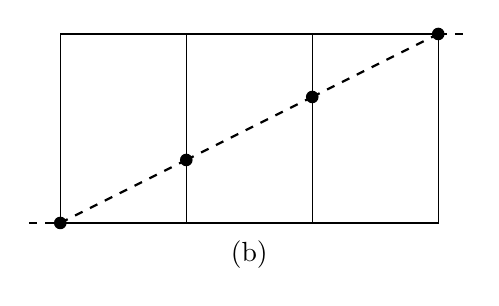
\begin{tikzpicture}[scale=0.8]
    \draw[dashed,thick] (-0.5,0) -- (0,0);
    \fill (0,0) circle (0.1);

    \draw (0,0) rectangle ++(2,3);
    \draw[dashed,thick] (0,0) -- ++(2,1);
    \fill (2,1) circle (0.1);

    \draw (2,0) rectangle ++(2,3);
    \draw[dashed,thick] (2,1) -- ++(2,1);
    \fill (4,2) circle (0.1);

    \draw (4,0) rectangle ++(2,3);
    \draw[dashed,thick] (4,2) -- ++(2,1);
    \fill (6,3) circle (0.1);

    \draw[dashed,thick] (6,3) -- (6.5,3);
    \node at (3, -1/2) {(b)};
  \end{tikzpicture}
  ~
  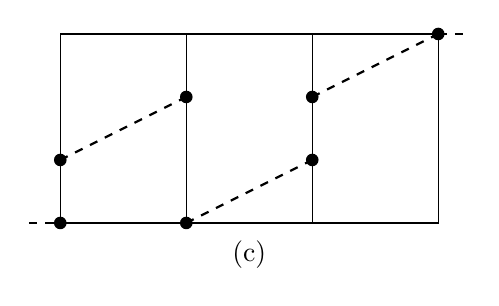
\begin{tikzpicture}[scale=0.8]
    \draw[dashed,thick] (-0.5,0) -- (0,0);
    \fill (0,0) circle (0.1);

    \draw (0,0) rectangle ++(2,3);
    \draw[dashed,thick] (0,1) -- ++(2,1);
    \fill (0,1) circle (0.1);
    \fill (2,2) circle (0.1);

    \draw (2,0) rectangle ++(2,3);
    \draw[dashed,thick] (2,0) -- ++(2,1);
    \fill (2,0) circle (0.1);
    \fill (4,1) circle (0.1);

    \draw (4,0) rectangle ++(2,3);
    \draw[dashed,thick] (4,2) -- ++(2,1);
    \fill (4,2) circle (0.1);
    \fill (6,3) circle (0.1);

    \draw[dashed,thick] (6,3) -- (6.5,3);
    \node at (3, -1/2) {(c)};
  \end{tikzpicture}
  \caption[A schematic for a switch that behaves like $S_3$.]{
    Part (a) shows a simple schematic for the components of a switch that
    behaves like $S_3$, the symmetric group on three letters.
    The three rectangles can be permuted arbitrarily, but only configuration (b)
    completes the circuit. All other configurations fail to
    complete the circuit (e.g., (c)).
  }
  \label{fig:S3Switch}
\end{figure}
